
\documentclass[11pt]{article}
\usepackage[a4paper,margin=1in]{geometry}
\usepackage[T1]{fontenc}
\usepackage[utf8]{inputenc}
\usepackage{lmodern,microtype}
\usepackage{amsmath,amssymb,amsthm,mathtools}
\usepackage{graphicx,booktabs,float,array,xcolor}
\usepackage[colorlinks=true,linkcolor=blue!60!black,citecolor=blue!60!black,urlcolor=blue!60!black]{hyperref}
\usepackage[nameinlink,capitalise,noabbrev]{cleveref}
\newtheorem{theorem}{Theorem}[section]
\newtheorem{proposition}[theorem]{Proposition}
\theoremstyle{definition}
\newtheorem{definition}[theorem]{Definition}
\newtheorem{remark}[theorem]{Remark}
\newcommand{\C}{\mathbb C}
\newcommand{\PP}{\mathbb P}
\newcommand{\R}{\mathbb R}
\newcommand{\PhiC}{\Phi_{\chi,B}}
\title{Projective Cubic Pandrosion by Finite-Slope Halley\\\large Completing Paper 0 bis with Riemann Inversion, Möbius Charts, Projective Scaling, and Dynamic Chart Changes}
\author{Ivan Besevic\\Independent Mathematical Research\\\texttt{github.com/ivan-fr/poussiere\_de\_x}}
\date{May 2026}
\begin{document}
\maketitle

\begin{abstract}
Paper 0 bis introduced a cubic finite-slope Halley-Pandrosion correction for scalar equations. The present version completes that note by inserting the missing global geometry from Paper 0 directly into the cubic method. The new algorithm does not merely choose a local probe radius. It first selects an active projective chart on the Riemann sphere, optionally applies inversion, applies a homothetic or projective scale, transports the equation to the chart coordinate, and only then performs the finite-slope Halley correction. In formulas, one solves $G(u)=f(\Phi_{\chi,B}(u))=0$ in a dynamically selected chart $\Phi_{\chi,B}$, computes symmetric finite slopes $D_1,D_2$ in that chart, updates by the cubic Halley-Pandrosion formula, and returns by $z=\Phi_{\chi,B}(u)$. Local theory shows that any stable biholomorphic chart preserves cubic order. Global theory shows that, for monomial targets, the dynamic chart rule is the same logarithmic homothety--inversion rule of Paper 0: choose the normalized target with smallest $|\log y|$. Benchmarks extend Paper 0 bis in two directions: a projective scaling benchmark over targets from $10^{-12}$ to $10^{12}$, and an extreme monomial benchmark showing that projective finite-slope Halley remains short and stable when the uncharted direct method is scale-sensitive.
\end{abstract}

\paragraph{One-sentence summary.} Paper 0 bis becomes a projective method when its cubic finite-slope Halley step is performed after dynamic Riemann-chart selection, inversion, and homothetic/projective scaling.

\section{Why 0 bis needs projective charts}
The original 0 bis note established the local hierarchy
\[
\text{raw finite slope} \quad\longrightarrow\quad \text{Steffensen quadratic} \quad\longrightarrow\quad \text{finite-slope Halley cubic}.
\]
However, local order is only one part of the Pandrosion philosophy. Paper 0 emphasized that the geometry should be normalized before iteration: a very large or very small target is not merely a hard number, but a number seen in the wrong chart. This paper therefore upgrades 0 bis by making the cubic correction explicitly charted.

The completed method has two layers:
\begin{enumerate}
\item a \emph{projective chart layer}: choose direct, inverse, or more general Möbius coordinates and scale them dynamically;
\item a \emph{local cubic layer}: run finite-slope Halley in the chosen chart coordinate.
\end{enumerate}

\begin{figure}[H]
\centering
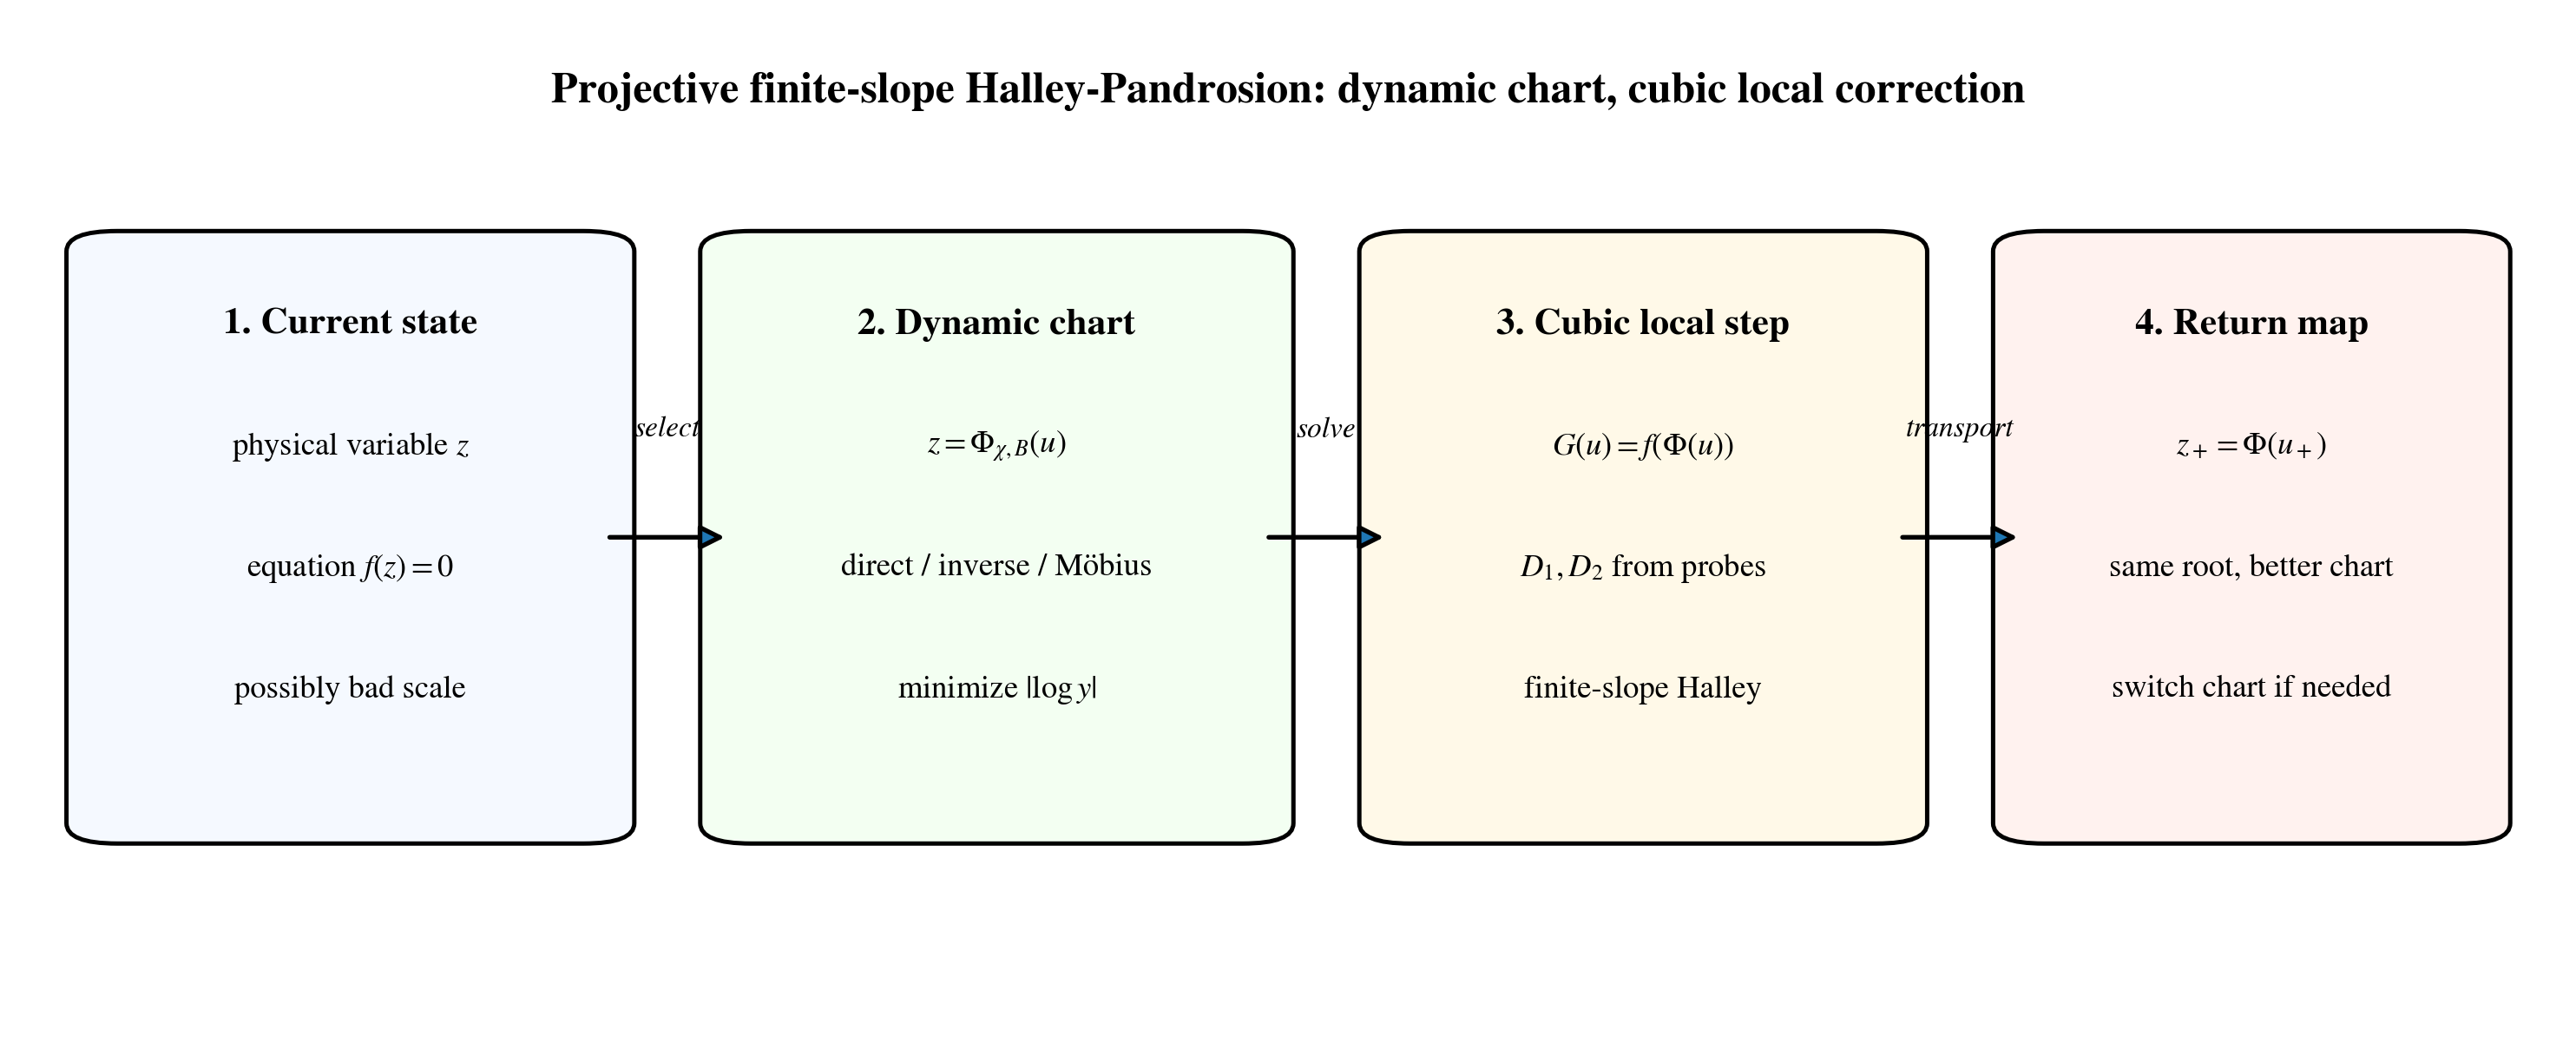
\includegraphics[width=.98\textwidth]{figures/fig_projective_pipeline.png}
\caption{Projective finite-slope Halley-Pandrosion. The equation is transported into an active chart, solved there by the cubic finite-slope correction, and returned to the original variable.}
\end{figure}

\section{Projective charts and Riemann inversion}
Let $f(z)=0$ be the scalar equation. A projective chart is a Möbius map
\[
\Phi(u)=\frac{au+b}{cu+d},\qquad ad-bc\neq0.
\]
The charted equation is
\[
G(u)=f(\Phi(u)).
\]
A root $u_*$ of $G$ gives a root $z_* = \Phi(u_*)$ of $f$.

Two special charts reproduce Paper 0 exactly.
\begin{description}
\item[Direct homothetic chart.] $z=Bu$. For $z^p=x$, this gives $u^p=x/B^p$.
\item[Reciprocal homothetic chart.] $z=1/(Bu)$. For $z^p=x$, this gives $u^p=1/(xB^p)$.
\end{description}
The second chart is Riemann inversion plus homothety. It is essential when the target is small in the original affine coordinate.

\begin{figure}[H]
\centering
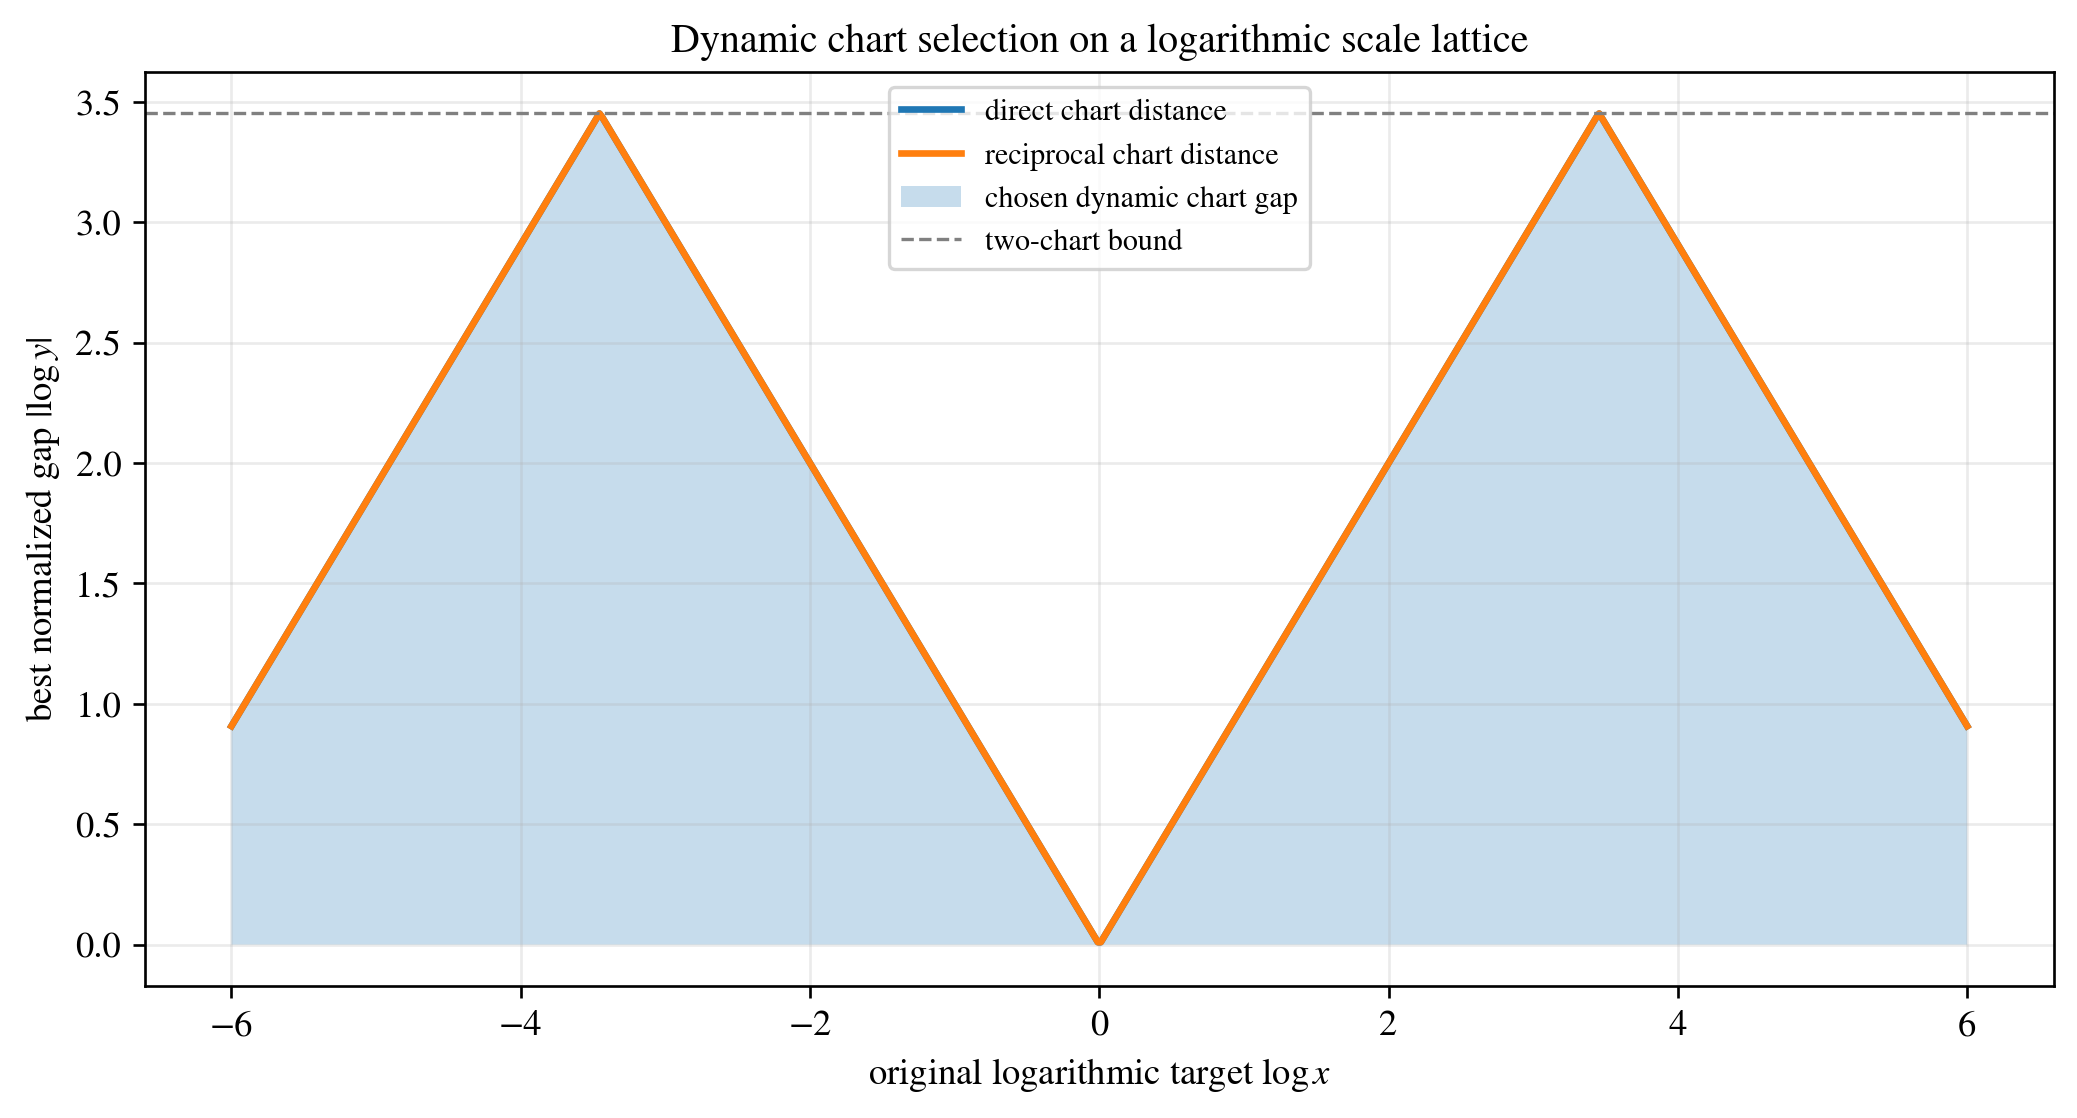
\includegraphics[width=.78\textwidth]{figures/fig_dynamic_chart_rule.png}
\caption{Dynamic chart selection as logarithmic scale selection. The direct and reciprocal charts provide complementary logarithmic gaps; the active chart is the one with the smallest normalized gap.}
\end{figure}

\section{Dynamic chart rule}
Fix a scale base $q>1$ and optional projective offsets $\omega_j\in[0,1)$. The available root scales are
\[
B=q^{m+\omega_j},\qquad m\in\mathbb Z.
\]
For $z^p=x$, define the direct and reciprocal normalized targets
\[
y_+(B)=\frac{x}{B^p},
\qquad
 y_\infty(B)=\frac{1}{xB^p}.
\]
The dynamic projective chart rule is
\begin{equation}
\label{eq:chart_rule}
(\chi,B)\in \arg\min_{\chi\in\{+,\infty\},B} |\log y_\chi(B)|,
\end{equation}
with the admissible branch $y_\chi(B)\ge1$ when one wants to use the exact monomial monotonicity theorem.

\begin{remark}
In a general non-monomial problem the same rule is replaced by a chart-quality functional involving residual norm, finite-slope conditioning, pole avoidance, and scale. The monomial case is special because $|\log y|$ is exactly tied to the raw multiplier.
\end{remark}

\section{Charted finite-slope Halley}
In an active chart $z=\Phi(u)$, define
\[
G(u)=f(\Phi(u)).
\]
The raw finite-slope predictor is
\[
\delta_{\rm raw}(u)=-\frac{G(u)}{G[u,u+h_0(u)]},
\qquad h_0(u)=\rho(1+|u|).
\]
Choose
\begin{equation}
\label{eq:h_charted}
h(u)=\eta\min(|\delta_{\rm raw}(u)|,h_0(u)).
\end{equation}
Then form the symmetric finite-slope surrogates in the chart coordinate:
\begin{equation}
D_1(u)=\frac{G(u+h(u))-G(u-h(u))}{2h(u)},
\qquad
D_2(u)=\frac{G(u+h(u))-2G(u)+G(u-h(u))}{h(u)^2}.
\end{equation}
The charted cubic finite-slope Halley-Pandrosion update is
\begin{equation}
\label{eq:charted_halley}
u_+ = u-\frac{2G(u)D_1(u)}{2D_1(u)^2-G(u)D_2(u)}.
\end{equation}
The returned physical iterate is
\[
z_+ = \Phi(u_+).
\]

\begin{figure}[H]
\centering
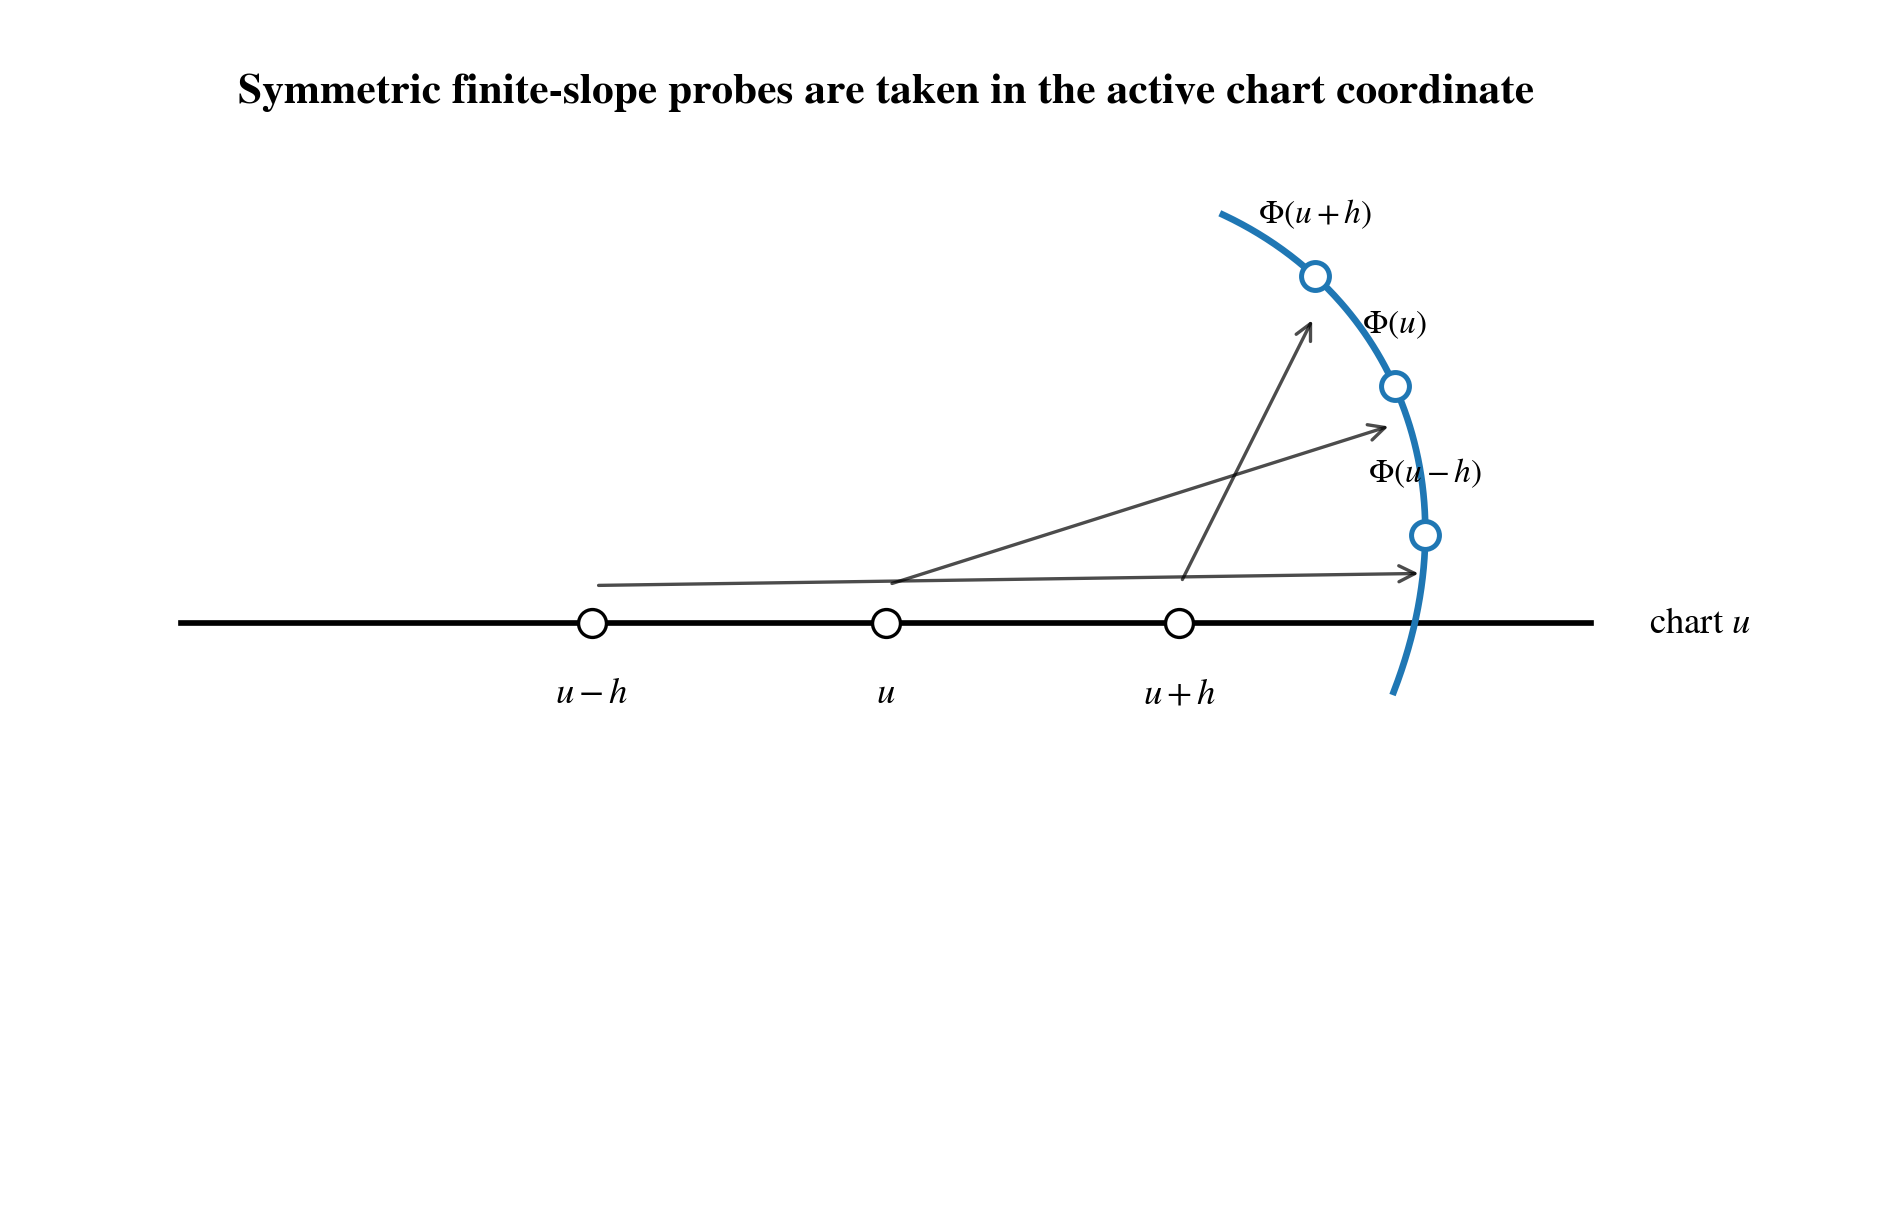
\includegraphics[width=.72\textwidth]{figures/fig_charted_symmetric_probes.png}
\caption{The symmetric probes $u-h,u,u+h$ are taken in the active chart coordinate. Their images under $\Phi$ need not be symmetric in the physical coordinate $z$. This is why the finite-slope Halley correction is truly charted.}
\end{figure}

\section{Dynamic chart changes}
A dynamic chart method may switch charts during an iteration. If the current chart is $\Phi_j$ and a step produces $u_j$, then the physical point is $z_j=\Phi_j(u_j)$. A new chart $\Phi_{j+1}$ is chosen by the chart-quality rule, and the same physical point is represented as
\[
u_{j+1}=\Phi_{j+1}^{-1}(z_j).
\]
The next finite-slope Halley step is then performed in the new coordinate.

This gives a simple invariant principle:
\begin{quote}
Changing chart changes coordinates, not the root being solved.
\end{quote}
In practice, one switches only when the chart quality deteriorates, for example when $|u|$ becomes too large, when $|\log y|$ becomes large in a monomial model, or when finite-slope conditioning worsens.

\section{Local theory}
The local cubic theorem of 0 bis survives charting.

\begin{proposition}[Charted cubic local convergence]
Let $f$ be analytic near a simple root $z_*$ and let $\Phi$ be a Möbius chart with $\Phi'(u_*)\neq0$ and $\Phi(u_*)=z_*$. Let $G(u)=f(\Phi(u))$. If the charted probe radius satisfies $h(u)=\Theta(u-u_*)$, then the update \cref{eq:charted_halley} satisfies
\[
u_+-u_* = C(u-u_*)^3+O((u-u_*)^4).
\]
Consequently,
\[
z_+-z_* = \Phi'(u_*)C(u-u_*)^3+O((u-u_*)^4),
\]
so the physical root coordinate is also cubic after the chart is fixed.
\end{proposition}

\begin{proof}[Proof sketch]
Since $\Phi$ is biholomorphic near $u_*$, the composed function $G=f\circ\Phi$ has a simple root at $u_*$. The scalar finite-slope Halley theorem from 0 bis applies to $G$. Finally, Taylor expansion of $\Phi$ transfers the cubic error estimate from $u$ to $z$.
\end{proof}

\begin{proposition}[Eventual cubic convergence under finite chart switching]
Suppose a dynamic chart algorithm performs only finitely many switches and eventually remains in a chart satisfying the hypotheses above. Then the subsequent convergence is cubic.
\end{proposition}

\section{Global monomial theory}
For monomial targets the chart-quality rule is exact. The raw monomial multiplier is
\[
\lambda_{p,y}=1-\frac{p}{S_p(y^{1/p})},
\qquad
S_p(\alpha)=1+\alpha+\cdots+\alpha^{p-1}.
\]
On the admissible branch $y\ge1$, the map $y\mapsto\lambda_{p,y}$ is strictly increasing. Therefore minimizing $|\log y|$ is equivalent to minimizing the exact raw multiplier.

With root-scale lattice $B=q^m$, direct scaling alone has worst-case normalized gap $p\log q$, while allowing the reciprocal chart halves the gap. With $K$ equally spaced offsets, the projective covering radius becomes
\[
\frac{p\log q}{2K},
\]
and the corresponding sharp minimax multiplier is
\begin{equation}
\label{eq:minimax}
1-\frac{p}{S_p(q^{1/(2K)})}.
\end{equation}
This is the same scaling theorem as Paper 0, now used as the global preconditioner for the cubic finite-slope Halley step.

\section{Benchmark I: projective scaling}
The first benchmark spans $x\in[10^{-12},10^{12}]$ and compares the raw one-chart multiplier against two-chart scaling and a four-offset projective palette.

\begin{figure}[H]
\centering
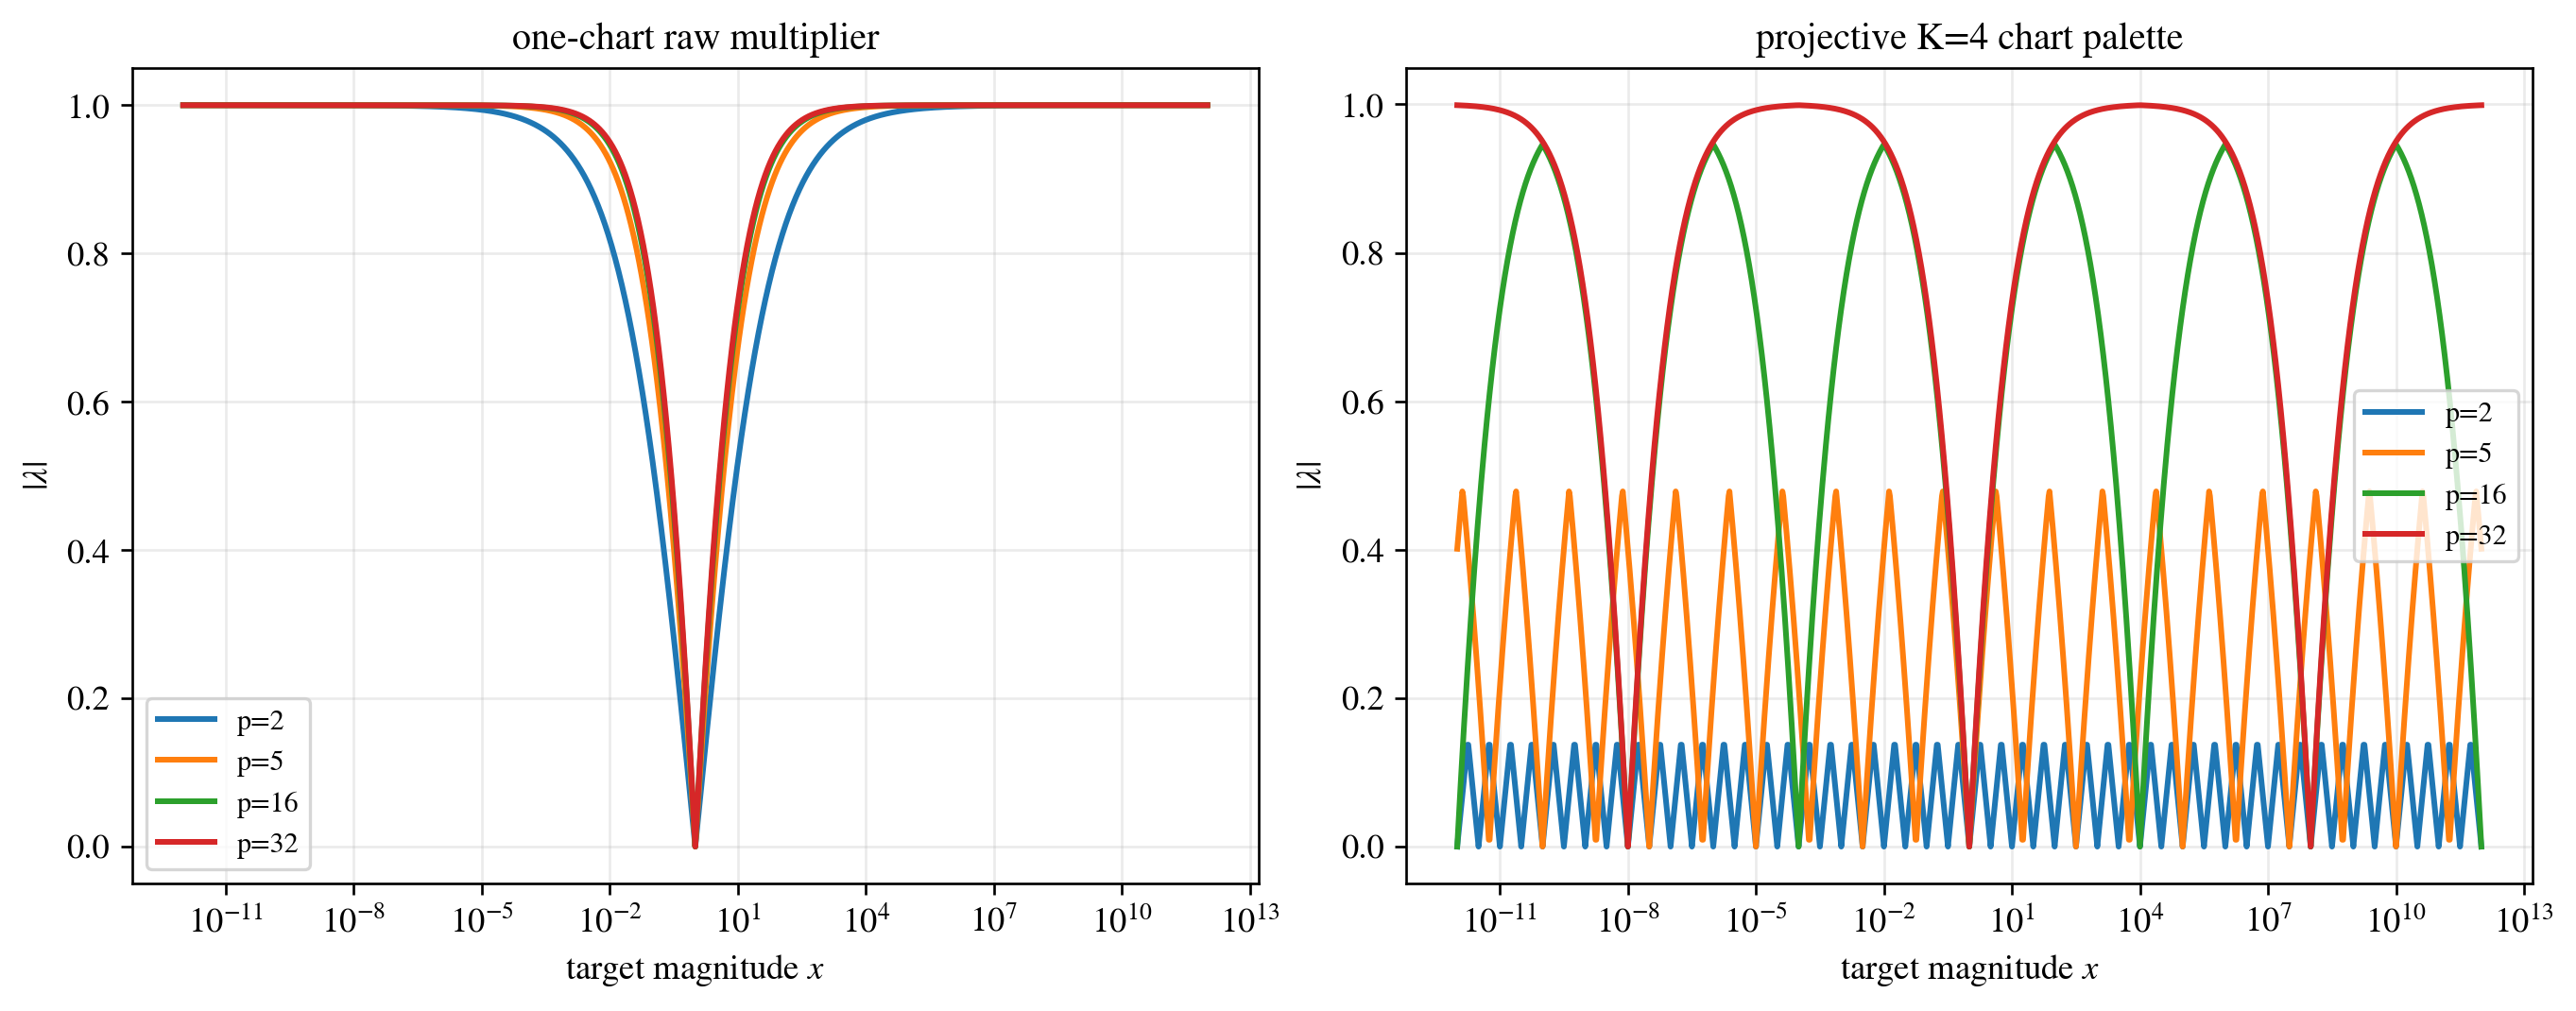
\includegraphics[width=.95\textwidth]{figures/fig_projective_scaling_benchmark.png}
\caption{Projective scaling benchmark. The four-offset projective chart palette keeps the normalized multiplier uniformly small over $24$ orders of magnitude in the original target.}
\end{figure}

\begin{table}[H]
\centering
\caption{Projective scaling summary over $x\in[10^{-12},10^{12}]$.}
\begin{tabular}{r r r r r}
\toprule
$p$ & max raw $|\lambda|$ & max two-chart $|\lambda|$ & max K=4 $|\lambda|$ & median K=4 $|\lambda|$\\
\midrule
2 & 1.0000 & 0.5195 & 0.1373 & 0.0690\\
3 & 1.0000 & 0.7882 & 0.2671 & 0.1418\\
5 & 1.0000 & 0.9657 & 0.4786 & 0.2712\\
8 & 1.0000 & 0.9983 & 0.7035 & 0.4273\\
16 & 1.0000 & 1.0000 & 0.9461 & 0.7248\\
32 & 1.0000 & 1.0000 & 0.9989 & 0.9500\\
\bottomrule
\end{tabular}
\end{table}

\section{Benchmark II: local cubic correction}
The second benchmark is the local 0 bis benchmark: three polynomial families, six degrees, $201$ starts per case, and the methods raw, Steffensen, and cubic finite-slope Halley.

\begin{figure}[H]
\centering
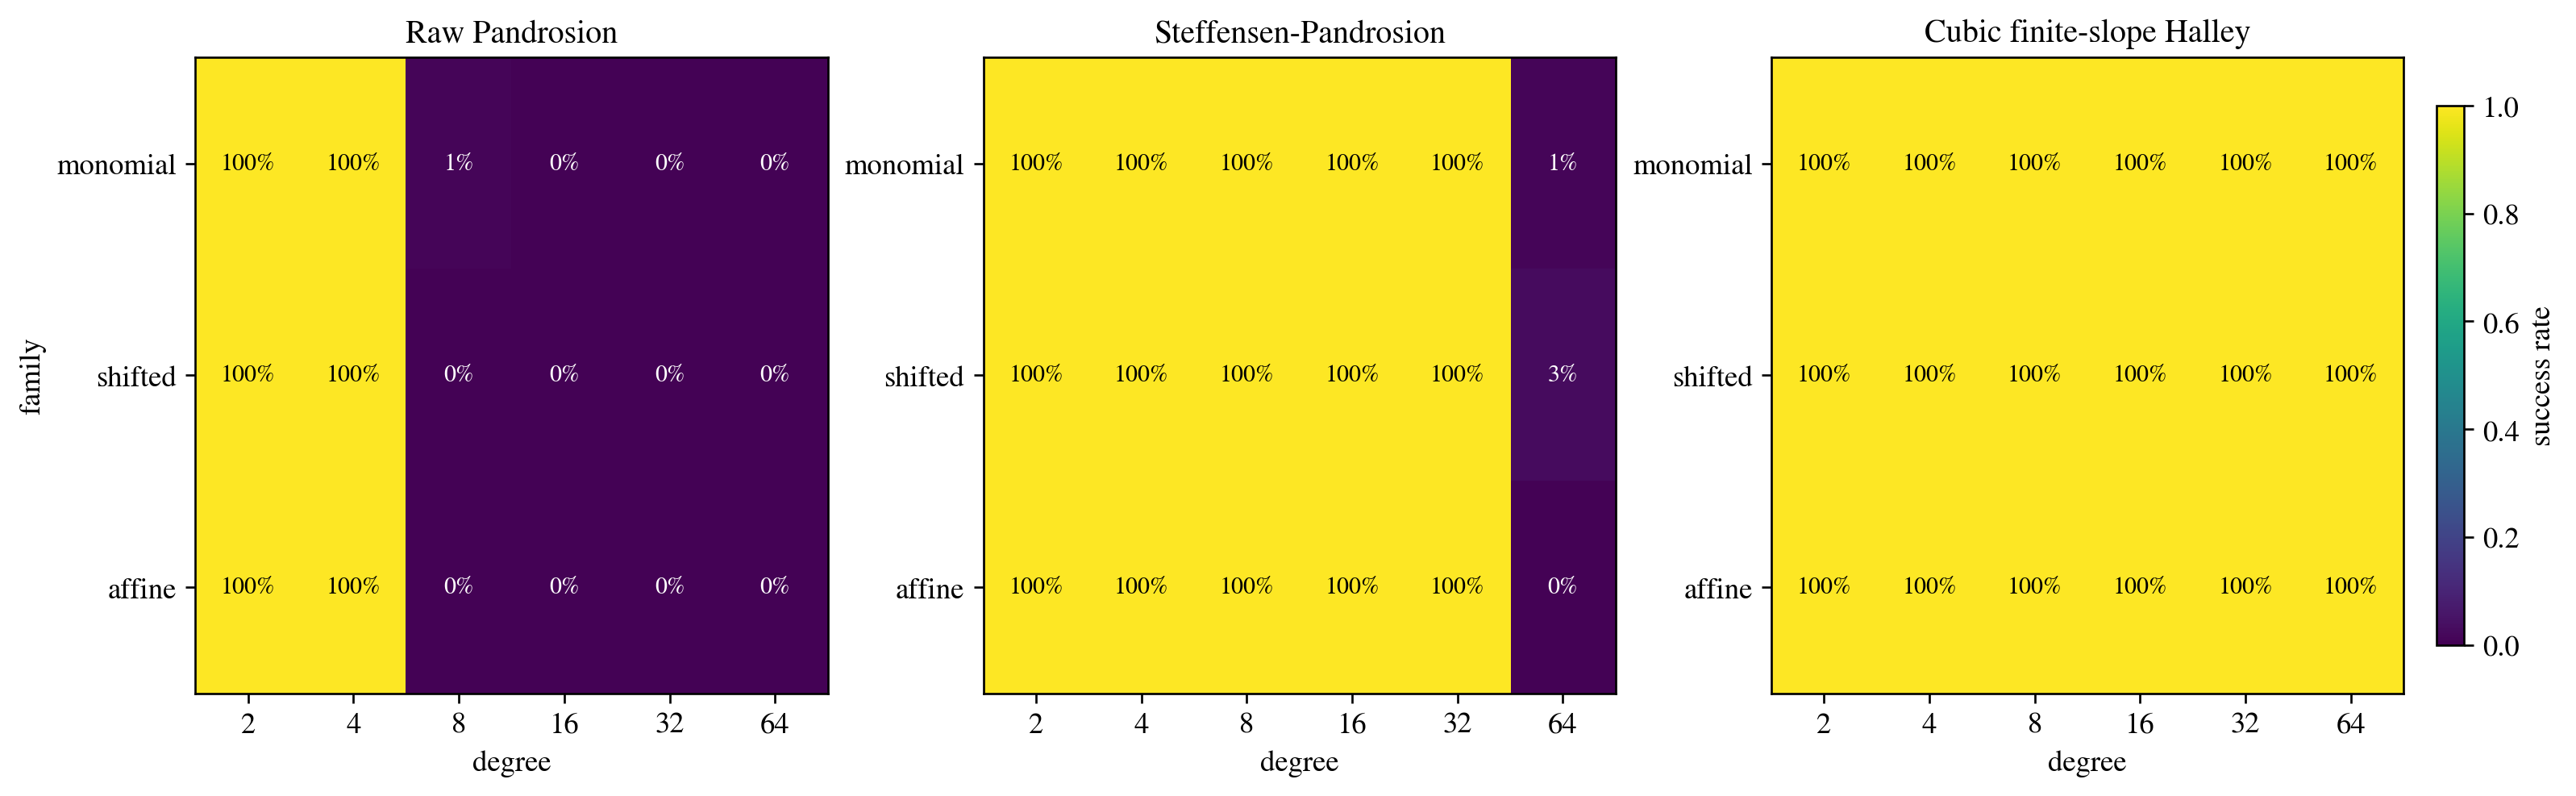
\includegraphics[width=.98\textwidth]{figures/fig_local_success_heatmaps.png}
\caption{Local benchmark success rates. The cubic finite-slope Halley correction keeps full success on the benchmark inherited from 0 bis.}
\end{figure}

\begin{table}[H]
\centering
\caption{Aggregate local benchmark summary, inherited from 0 bis.}
\begin{tabular}{r l r r r}
\toprule
Degree & Method & mean success & median iters & median evals\\
\midrule
2 & Raw Pandrosion & 100.0\% & 10 & 31\\
2 & Steffensen-Pandrosion & 100.0\% & 3 & 16\\
2 & Cubic finite-slope Halley & 100.0\% & 2 & 11\\
4 & Raw Pandrosion & 100.0\% & 18 & 55\\
4 & Steffensen-Pandrosion & 100.0\% & 3 & 16\\
4 & Cubic finite-slope Halley & 100.0\% & 2 & 11\\
8 & Raw Pandrosion & 0.8\% & 0 & 1\\
8 & Steffensen-Pandrosion & 100.0\% & 4 & 21\\
8 & Cubic finite-slope Halley & 100.0\% & 3 & 16\\
16 & Raw Pandrosion & 0.5\% & 0 & 1\\
16 & Steffensen-Pandrosion & 100.0\% & 4 & 21\\
16 & Cubic finite-slope Halley & 100.0\% & 3 & 16\\
32 & Raw Pandrosion & 0.5\% & 0 & 1\\
32 & Steffensen-Pandrosion & 100.0\% & 6 & 31\\
32 & Cubic finite-slope Halley & 100.0\% & 3 & 16\\
64 & Raw Pandrosion & 0.5\% & 0 & 1\\
64 & Steffensen-Pandrosion & 1.7\% & 5 & 26\\
64 & Cubic finite-slope Halley & 100.0\% & 4 & 21\\
\bottomrule
\end{tabular}
\end{table}

\section{Benchmark III: extreme projective Halley targets}
The final benchmark applies finite-slope Halley to extreme monomial targets. The direct method solves $z^p=x$ from $z_0=1$. The projective method first chooses a dynamic projective chart from four offsets, solves $u^p=y$ near $y\approx1$, and returns by the chart map.

\begin{figure}[H]
\centering
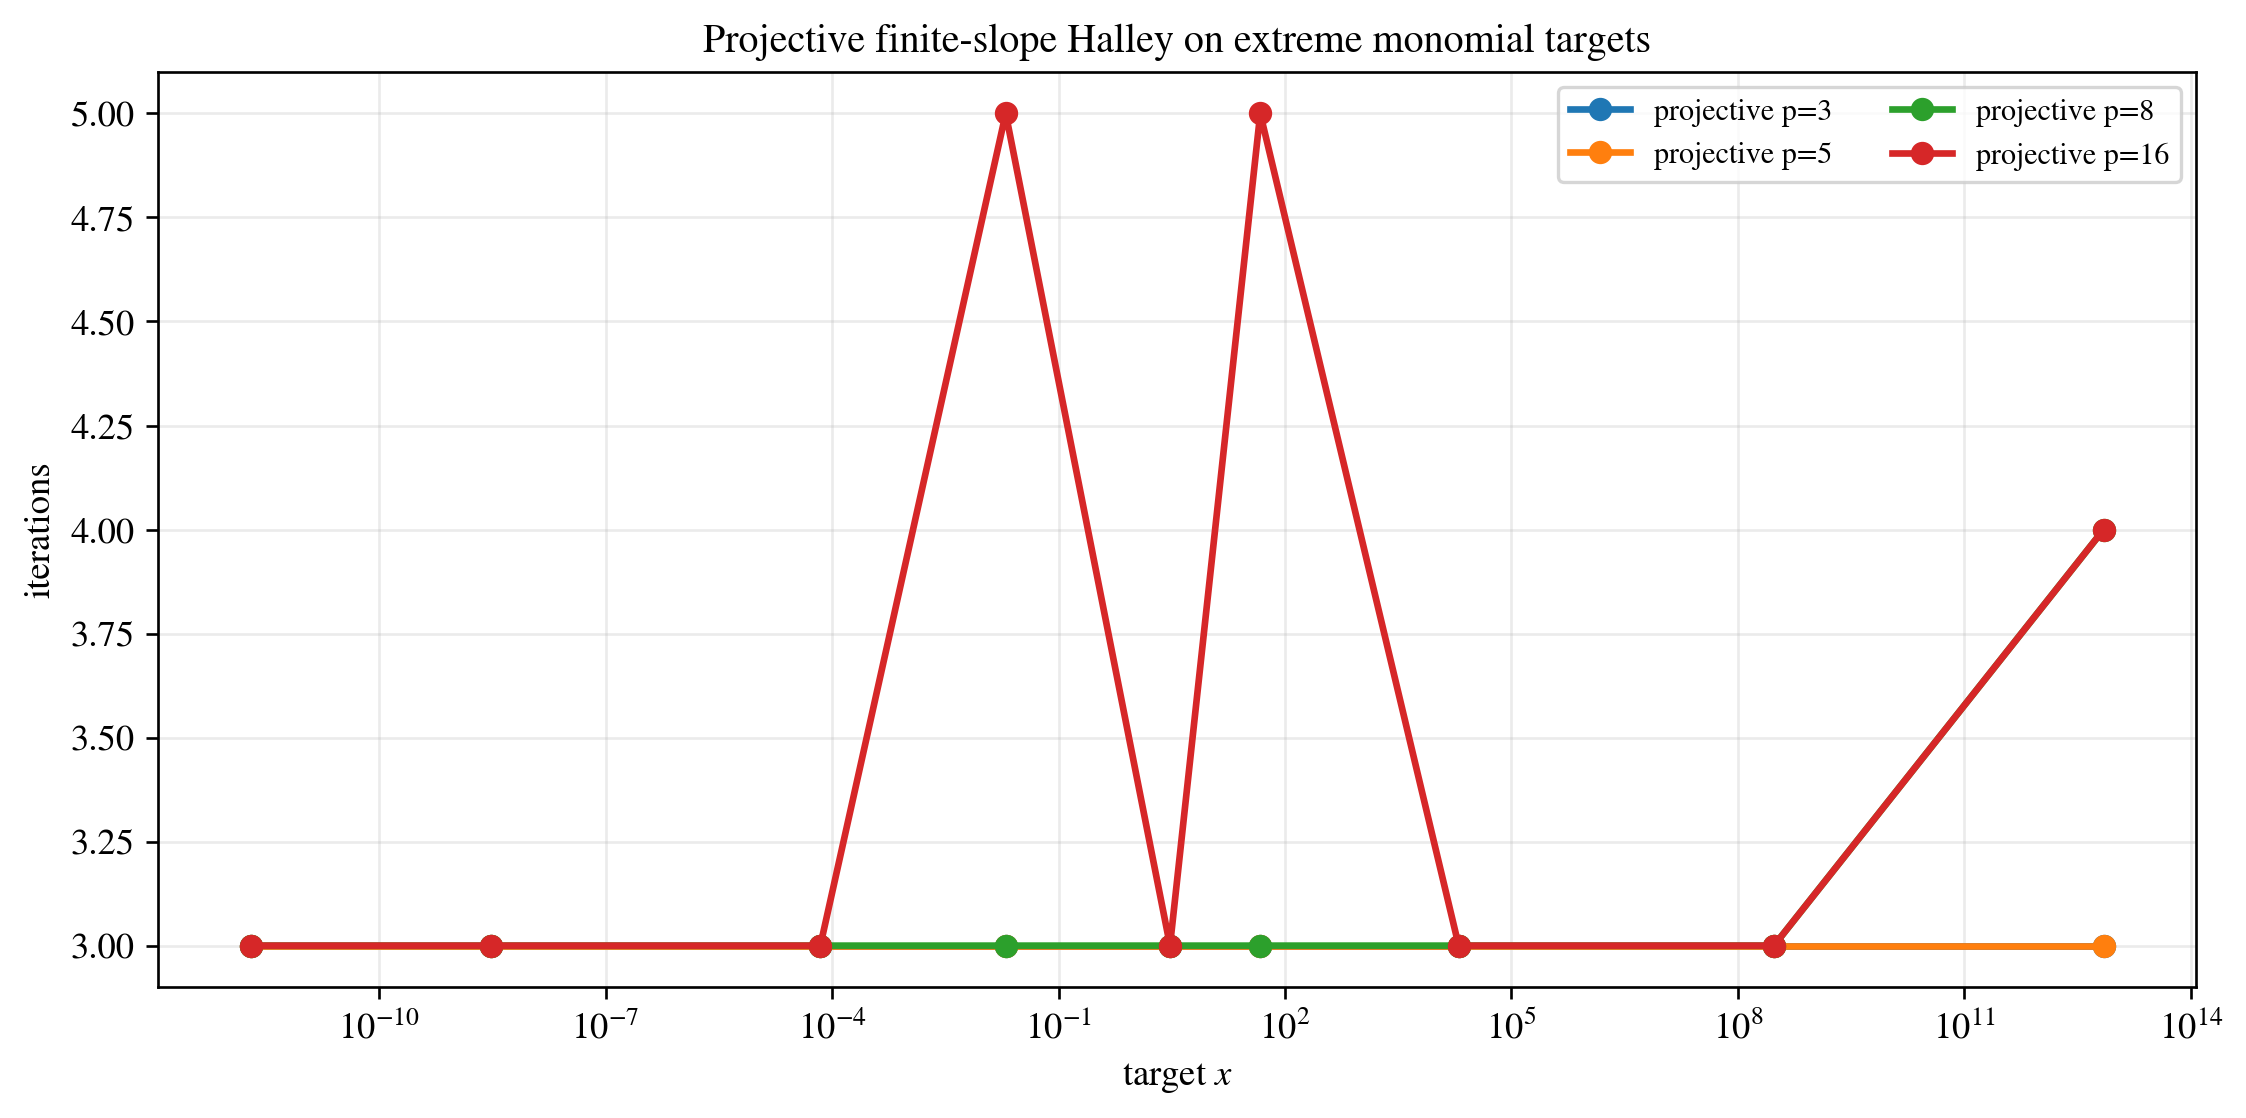
\includegraphics[width=.82\textwidth]{figures/fig_projective_iters.png}
\caption{Projective finite-slope Halley on extreme monomial targets. After projective chart selection, iteration counts remain small across many orders of magnitude in $x$.}
\end{figure}

\begin{table}[H]
\centering
\caption{Extreme target benchmark summary.}
\begin{tabular}{r r r r r}
\toprule
$p$ & direct success & projective success & projective median iters & projective median evals\\
\midrule
3 & 100.0\% & 100.0\% & 3 & 16\\
5 & 88.9\% & 100.0\% & 3 & 16\\
8 & 88.9\% & 100.0\% & 3 & 16\\
16 & 88.9\% & 100.0\% & 3 & 16\\
\bottomrule
\end{tabular}
\end{table}

\section{Discussion}
The completed 0 bis paper makes the finite-slope Halley correction explicitly Pandrosion-geometric in the sense of Paper 0. The probe radius is not only local; the active coordinate system is also selected geometrically. Inversion, homothety, projective scaling, and chart return are all part of the method, not preprocessing decorations.

The most important practical rule is:
\[
\boxed{\text{choose the projective chart globally, then apply cubic finite-slope Halley locally.}}
\]

\section{Limitations}
This paper remains scalar. The multivariate version would require replacing the scalar $D_2$ by a finite-slope second-order tensor or by a two-stage vector Halley correction. Nevertheless, the scalar charted theory gives the correct design principle for future engines such as a 131+Halley successor: branchless/projective charting globally, cubic finite-slope correction locally.

\section{Conclusion}
The original 0 bis note showed that raw Pandrosion can be upgraded to cubic local behavior by a derivative-free finite-slope Halley correction. The completed version shows where that correction belongs in the full Paper 0 geometry: inside a dynamic projective chart, after homothety and Riemann inversion have normalized the target. The resulting method is both global and local: global through chart scaling, local through cubic finite-slope Halley.

\begin{thebibliography}{9}
\bibitem{halley} E. Halley, \emph{A new, exact, and easy method of finding the roots of equations generally}, Philosophical Transactions, 1694.
\bibitem{householder} A. S. Householder, \emph{The Numerical Treatment of a Single Nonlinear Equation}, McGraw--Hill, 1970.
\bibitem{traub} J. F. Traub, \emph{Iterative Methods for the Solution of Equations}, Prentice--Hall, 1964.
\bibitem{milnor} J. Milnor, \emph{Dynamics in One Complex Variable}, Princeton University Press, 2006.
\bibitem{pand0} I. Besevic, \emph{A Monomial Pandrosion Scheme}, manuscript, 2026.
\bibitem{pand0bis} I. Besevic, \emph{Paper 0 bis: Cubic Pandrosion by Finite-Slope Halley Acceleration}, manuscript, 2026.
\end{thebibliography}
\end{document}
